\documentclass[notes,11pt, aspectratio=169, xcolor=table]{beamer}

\usepackage{pgfpages}
% These slides also contain speaker notes. You can print just the slides,
% just the notes, or both, depending on the setting below. Comment out the want
% you want.
\setbeameroption{hide notes} % Only slide
%\setbeameroption{show only notes} % Only notes
%\setbeameroption{show notes on second screen=right} % Both

\usepackage{helvet}
\usepackage[default]{lato}
\usepackage{array}
\usepackage[utf8]{inputenc} 

\newtheorem{proposition}{Proposition}

\usepackage{tikz}
\usetikzlibrary{shapes.geometric}
\usepackage{pgfplots}
\usepackage{graphicx}
\usepackage{verbatim}
\setbeamertemplate{note page}{\pagecolor{yellow!5}\insertnote}
\usetikzlibrary{positioning}
\usetikzlibrary{snakes}
\usetikzlibrary{calc}
\usetikzlibrary{arrows}
\usetikzlibrary{decorations.markings}
\usetikzlibrary{shapes.misc}
\usetikzlibrary{matrix,shapes,arrows,fit,tikzmark}
\usepackage{amsmath}
\usepackage{mathpazo}
\usepackage{hyperref}
\usepackage{lipsum}
\usepackage{multimedia}
\usepackage{graphicx}
\usepackage{multirow}
\usepackage{graphicx}
\usepackage{dcolumn}
\usepackage{bbm}
\usepackage[style=authoryear,sorting=nyt,uniquename=false]{biblatex}

\addbibresource{references.bib} 

\newcolumntype{d}[0]{D{.}{.}{5}}

\def\@@mybluebox[#1][#2]#3{
    \sbox\mytempbox{#3}%
    \mytemplen\ht\mytempbox
    \advance\mytemplen #1\relax
    \ht\mytempbox\mytemplen
    \mytemplen\dp\mytempbox
    \advance\mytemplen #2\relax
    \dp\mytempbox\mytemplen
    \colorbox{myblue}{\hspace{1em}\usebox{\mytempbox}\hspace{1em}}}


\usepackage{changepage}
\usepackage{appendixnumberbeamer}
\newcommand{\beginbackup}{
   \newcounter{framenumbervorappendix}
   \setcounter{framenumbervorappendix}{\value{framenumber}}
   \setbeamertemplate{footline}
   {
     \leavevmode%
     \hline
     box{%
       \begin{beamercolorbox}[wd=\paperwidth,ht=2.25ex,dp=1ex,right]{footlinecolor}%
%         \insertframenumber  \hspace*{2ex} 
       \end{beamercolorbox}}%
     \vskip0pt%
   }
 }
\newcommand{\backupend}{
   \addtocounter{framenumbervorappendix}{-\value{framenumber}}
   \addtocounter{framenumber}{\value{framenumbervorappendix}} 
}


\usepackage{graphicx}
\usepackage[space]{grffile}
\usepackage{booktabs}

% These are my colors -- there are many like them, but these ones are mine.
\definecolor{blue}{RGB}{0,114,178}
\definecolor{red}{RGB}{213,94,0}
\definecolor{yellow}{RGB}{240,228,66}
\definecolor{green}{RGB}{0,158,115}

\hypersetup{
  colorlinks=false,
  linkbordercolor = {white},
  linkcolor = {blue}
}


%% I use a beige off white for my background
\definecolor{MyBackground}{RGB}{255,253,218}

%% Uncomment this if you want to change the background color to something else
%\setbeamercolor{background canvas}{bg=MyBackground}

%% Change the bg color to adjust your transition slide background color!
\newenvironment{transitionframe}{
  \setbeamercolor{background canvas}{bg=yellow}
  \begin{frame}}{
    \end{frame}
}

\setbeamercolor{frametitle}{fg=blue}
\setbeamercolor{title}{fg=blue}
\setbeamertemplate{footline}[frame number]
\setbeamertemplate{navigation symbols}{} 
\setbeamertemplate{itemize items}{-}
\setbeamercolor{itemize item}{fg=blue}
\setbeamercolor{itemize subitem}{fg=blue}
\setbeamercolor{enumerate item}{fg=blue}
\setbeamercolor{enumerate subitem}{fg=blue}
\setbeamercolor{button}{bg=MyBackground,fg=blue,}



% If you like road maps, rather than having clutter at the top, have a roadmap show up at the end of each section 
% (and after your introduction)
% Uncomment this is if you want the roadmap!
% \AtBeginSection[]
% {
%    \begin{frame}
%        \frametitle{Roadmap of Talk}
%        \tableofcontents[currentsection]
%    \end{frame}
% }
\setbeamercolor{section in toc}{fg=blue}
\setbeamercolor{subsection in toc}{fg=red}
\setbeamersize{text margin left=1em,text margin right=1em} 

\newenvironment{wideitemize}{\itemize\addtolength{\itemsep}{10pt}}{\enditemize}

\usepackage{environ}
\NewEnviron{videoframe}[1]{
  \begin{frame}
    \vspace{-8pt}
    \begin{columns}[onlytextwidth, T] % align columns
      \begin{column}{.58\textwidth}
        \begin{minipage}[t][\textheight][t]
          {\dimexpr\textwidth}
          \vspace{8pt}
          \hspace{4pt} {\Large \sc \textcolor{blue}{#1}}
          \vspace{8pt}
          
          \BODY
        \end{minipage}
      \end{column}%
      \hfill%
      \begin{column}{.42\textwidth}
        \colorbox{green!20}{\begin{minipage}[t][1.2\textheight][t]
            {\dimexpr\textwidth}
            Face goes here
          \end{minipage}}
      \end{column}%
    \end{columns}
  \end{frame}
}

\title[]{International Trade: Lecture XX}
\subtitle[]{Economies of Scale}
\author[Góes]
{Carlos Góes\inst{1}}
\date{Fall 2025}
\institute[GWU]{\inst{1} George Washington University }



\begin{document}

%%% TIKZ STUFF
\tikzset{   
        every picture/.style={remember picture,baseline},
        every node/.style={anchor=base,align=center,outer sep=1.5pt},
        every path/.style={thick},
        }
\newcommand\marktopleft[1]{%
    \tikz[overlay,remember picture] 
        \node (marker-#1-a) at (-.3em,.3em) {};%
}
\newcommand\markbottomright[2]{%
    \tikz[overlay,remember picture] 
        \node (marker-#1-b) at (0em,0em) {};%
}
\tikzstyle{every picture}+=[remember picture] 
\tikzstyle{mybox} =[draw=black, very thick, rectangle, inner sep=10pt, inner ysep=20pt]
\tikzstyle{fancytitle} =[draw=black,fill=red, text=white]
%%%% END TIKZ STUFF



%----------------------------------------------------------------------%
%-------------------       TITLE PAGE       ---------------------------%
%----------------------------------------------------------------------%





%----------------------------------------------------------------------%






%----------------------------------------------------------------------%
%----------------------------------------------------------------------%

%----------------------------------------------------------------------%
\frame{\titlepage}
\addtocounter{framenumber}{-1}
%----------------------------------------------------------------------%



%----------------------------------------------------------------------%
%----------------------------------------------------------------------%

\begin{frame}{Motivation}
\begin{wideitemize}
    \item The models of comparative advantage we saw assumed constant returns to scale. 
    
    \item If inputs to an industry were doubled, industry output would double as well.
    
    \item Many industries
are characterized by economies of scale (aka increasing returns)

\item Production is more efficient the larger the scale at which it takes place.

\item Can we think of examples?
\end{wideitemize}
    
\end{frame}

\begin{frame}{Economies of Scale}

\begin{wideitemize}
    
    \item \textbf{Internal economies of scale} occur when the cost per unit depends on the size of an individual firm but not necessarily on that of the industry.
    \\ \qquad (fixed costs, specific human capital) 
    
    \item<2-> \textbf{External economies of scale} occur when the cost per unit depends on the size of the industry but not necessarily on the size of any one firm.
    \\ \qquad (specialized suppliers; labor market pooling; knowledge spillovers)

    \item<3-> Suppose an economy produces 1000 thneeds, with each of 10 firms producing 100

    \begin{itemize}
        \item If costs in each firm decrease if total production goes to 2000 with 20 firms producing 100 each, we have external economies of scale
        \item If costs in each firm decrease if production per firm increases to 200 each, with 5 firms producing in total producing 1000, we have internal economies of scale
    \end{itemize}

    \item<4-> Although the mechanisms differ, they generate a similar intuition: the long-run equilibrium cost curve slopes downward in both cases.


\end{wideitemize}
    
\end{frame}

\begin{frame}{Fixed costs and increasing returns}
\blue{Consider the production of a \textbf{new drug}}
\normalsize
\begin{wideitemize}
    \item there is a large \textbf{fixed cost investment} $\bar{f}$ of \$2.5 billion to develop and get approval 
    \item<2-> after the drug is developed and approved, producing new doses can be produced with a constant marginal cost: each 100 doses cost \$10 to produce
    
\end{wideitemize}

\onslide<3->{


\begin{columns}[T] % align columns
\begin{column}{.45\textwidth}
            \centering
    \vspace{18pt}
    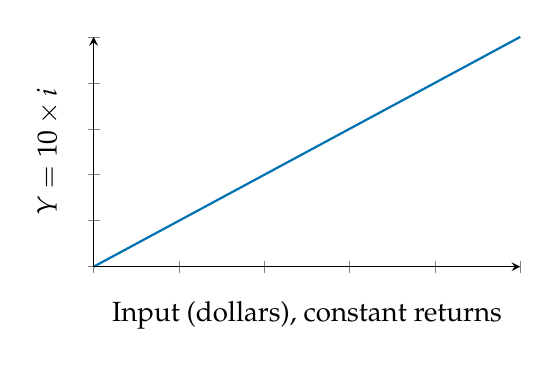
\begin{tikzpicture}

    \pgfmathsetmacro{\m}{10}


    
    \centering
    \begin{axis}[
        ylabel={$Y = 10 \times i$},
        xlabel={Input (dollars), constant returns},
        ymin=0, ymax=10,
        xmin=0, xmax=1,
        yticklabel=\empty,
        xticklabel=\empty,
        axis lines=left,
        enlargelimits=false,
        clip=false,
        axis on top,
        scaled x ticks=false,
        width=7cm, height=4.5cm,
        title style={font=\bfseries}
    ]
    
    % PPF: Q_C = (L/a_C) - (a_R/a_C) * Q_R
    \addplot[blue, thick, domain=0:1] {\m * x};


    %\node[anchor = west] at (axis cs:\Qc, {\Yt + (\Qt-\Yt)/2}) {\scriptsize Exports};
    
    \end{axis}

\end{tikzpicture}

                
    \end{column}
    \begin{column}{.45\textwidth}

    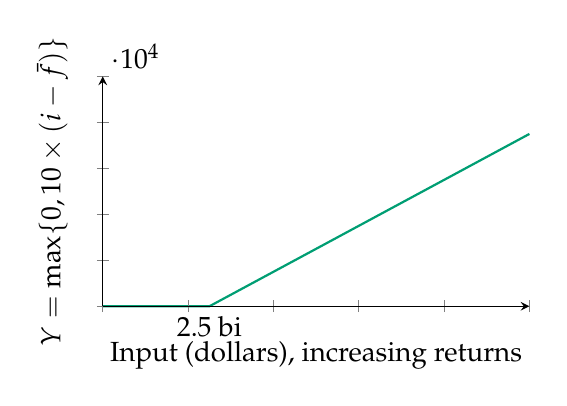
\begin{tikzpicture}
    \pgfmathsetmacro{\m}{10}
    \pgfmathsetmacro{\f}{250}

    
    
    \centering
    \begin{axis}[
        ylabel={$Y = \max\{ 0, 10 \times (i-\bar{f}) \}$},
        xlabel={Input (dollars), increasing returns},
        ymin=0, ymax=10000,
        xmin=0, xmax=1000,
        yticklabel=\empty,
        xticklabel=\empty,
        axis lines=left,
        enlargelimits=false,
        clip=false,
        axis on top,
        scaled x ticks=false,
        width=7cm, height=4.5cm,
        title style={font=\bfseries}
    ]

        \addplot[green, thick, domain=0:1000] {max(0,\m * (x-\f))};

        \node[anchor = north] at (axis cs: 250, 0) {$2.5$ bi};


    \end{axis}

\end{tikzpicture}

\end{column}
\end{columns}


}

\end{frame}

\begin{frame}{Fixed costs and increasing returns}
\Large Consider the production of a \textbf{new drug}.
\normalsize
\begin{wideitemize}
    \item Decreasing average cost
\end{wideitemize}


    \onslide<2->{
    \centering
    \begin{tikzpicture}
    \pgfmathsetmacro{\m}{1}
    \pgfmathsetmacro{\f}{2.5}

    
    
    \begin{axis}[
        ylabel={$AC = 1/10 + \bar{f}/Y$},
        xlabel={Output $Y$},
        ymin=0, ymax=10,
        xmin=0, xmax=10,
        yticklabel=\empty,
        xticklabel=\empty,
        axis lines=left,
        enlargelimits=false,
        clip=false,
        axis on top,
        scaled x ticks=false,
        width=7cm, height=7cm,
        title style={font=\bfseries}
    ]

        \addplot[green, thick, domain=0.3:10] {1/\m + \f / x};
        \addplot[black, thick, domain=0:10] {1/\m};

    \end{axis}

\end{tikzpicture}

}
\end{frame}




\begin{frame}{Increasing returns and trade}
\normalsize

\begin{columns}[T] % align columns
\begin{column}{.45\textwidth}

        \begin{wideitemize}
    \item Economies of scale provide an incentive for international trade.
    \item<2-> Imagine a small country, like Denmark
    \item<3-> Its 6 million population provides limited scale
    \item<4-> It would be hard to justify spending \$ 5 billion on a new drug
    \item<5-> Yet... it happened!
    \item<7-> Trade provides a vehicle for scale and innovation
    
\end{wideitemize}
            
                
    \end{column}
    \begin{column}{.45\textwidth}

    \onslide<6-> {

    \begin{figure}
        \centering
        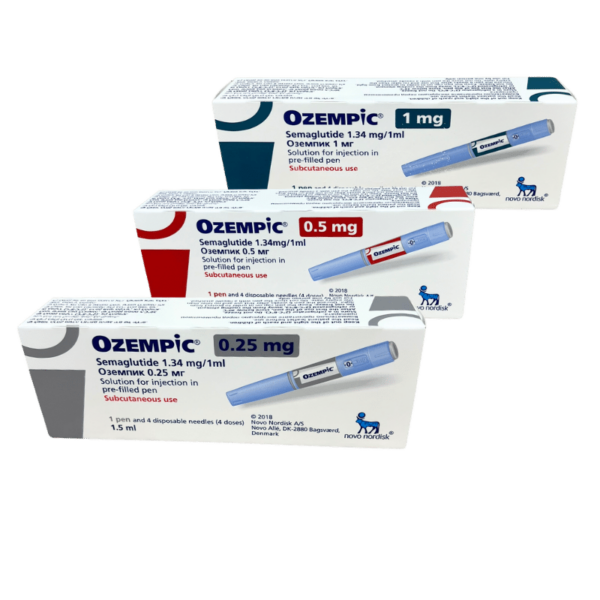
\includegraphics[width=\linewidth]{figs/Ozempic025051-1-600x600.png}
    \end{figure}

    
    }

\end{column}
\end{columns}




\end{frame}

\begin{frame}{Increasing returns and trade}
\normalsize

\begin{figure}
    \centering
    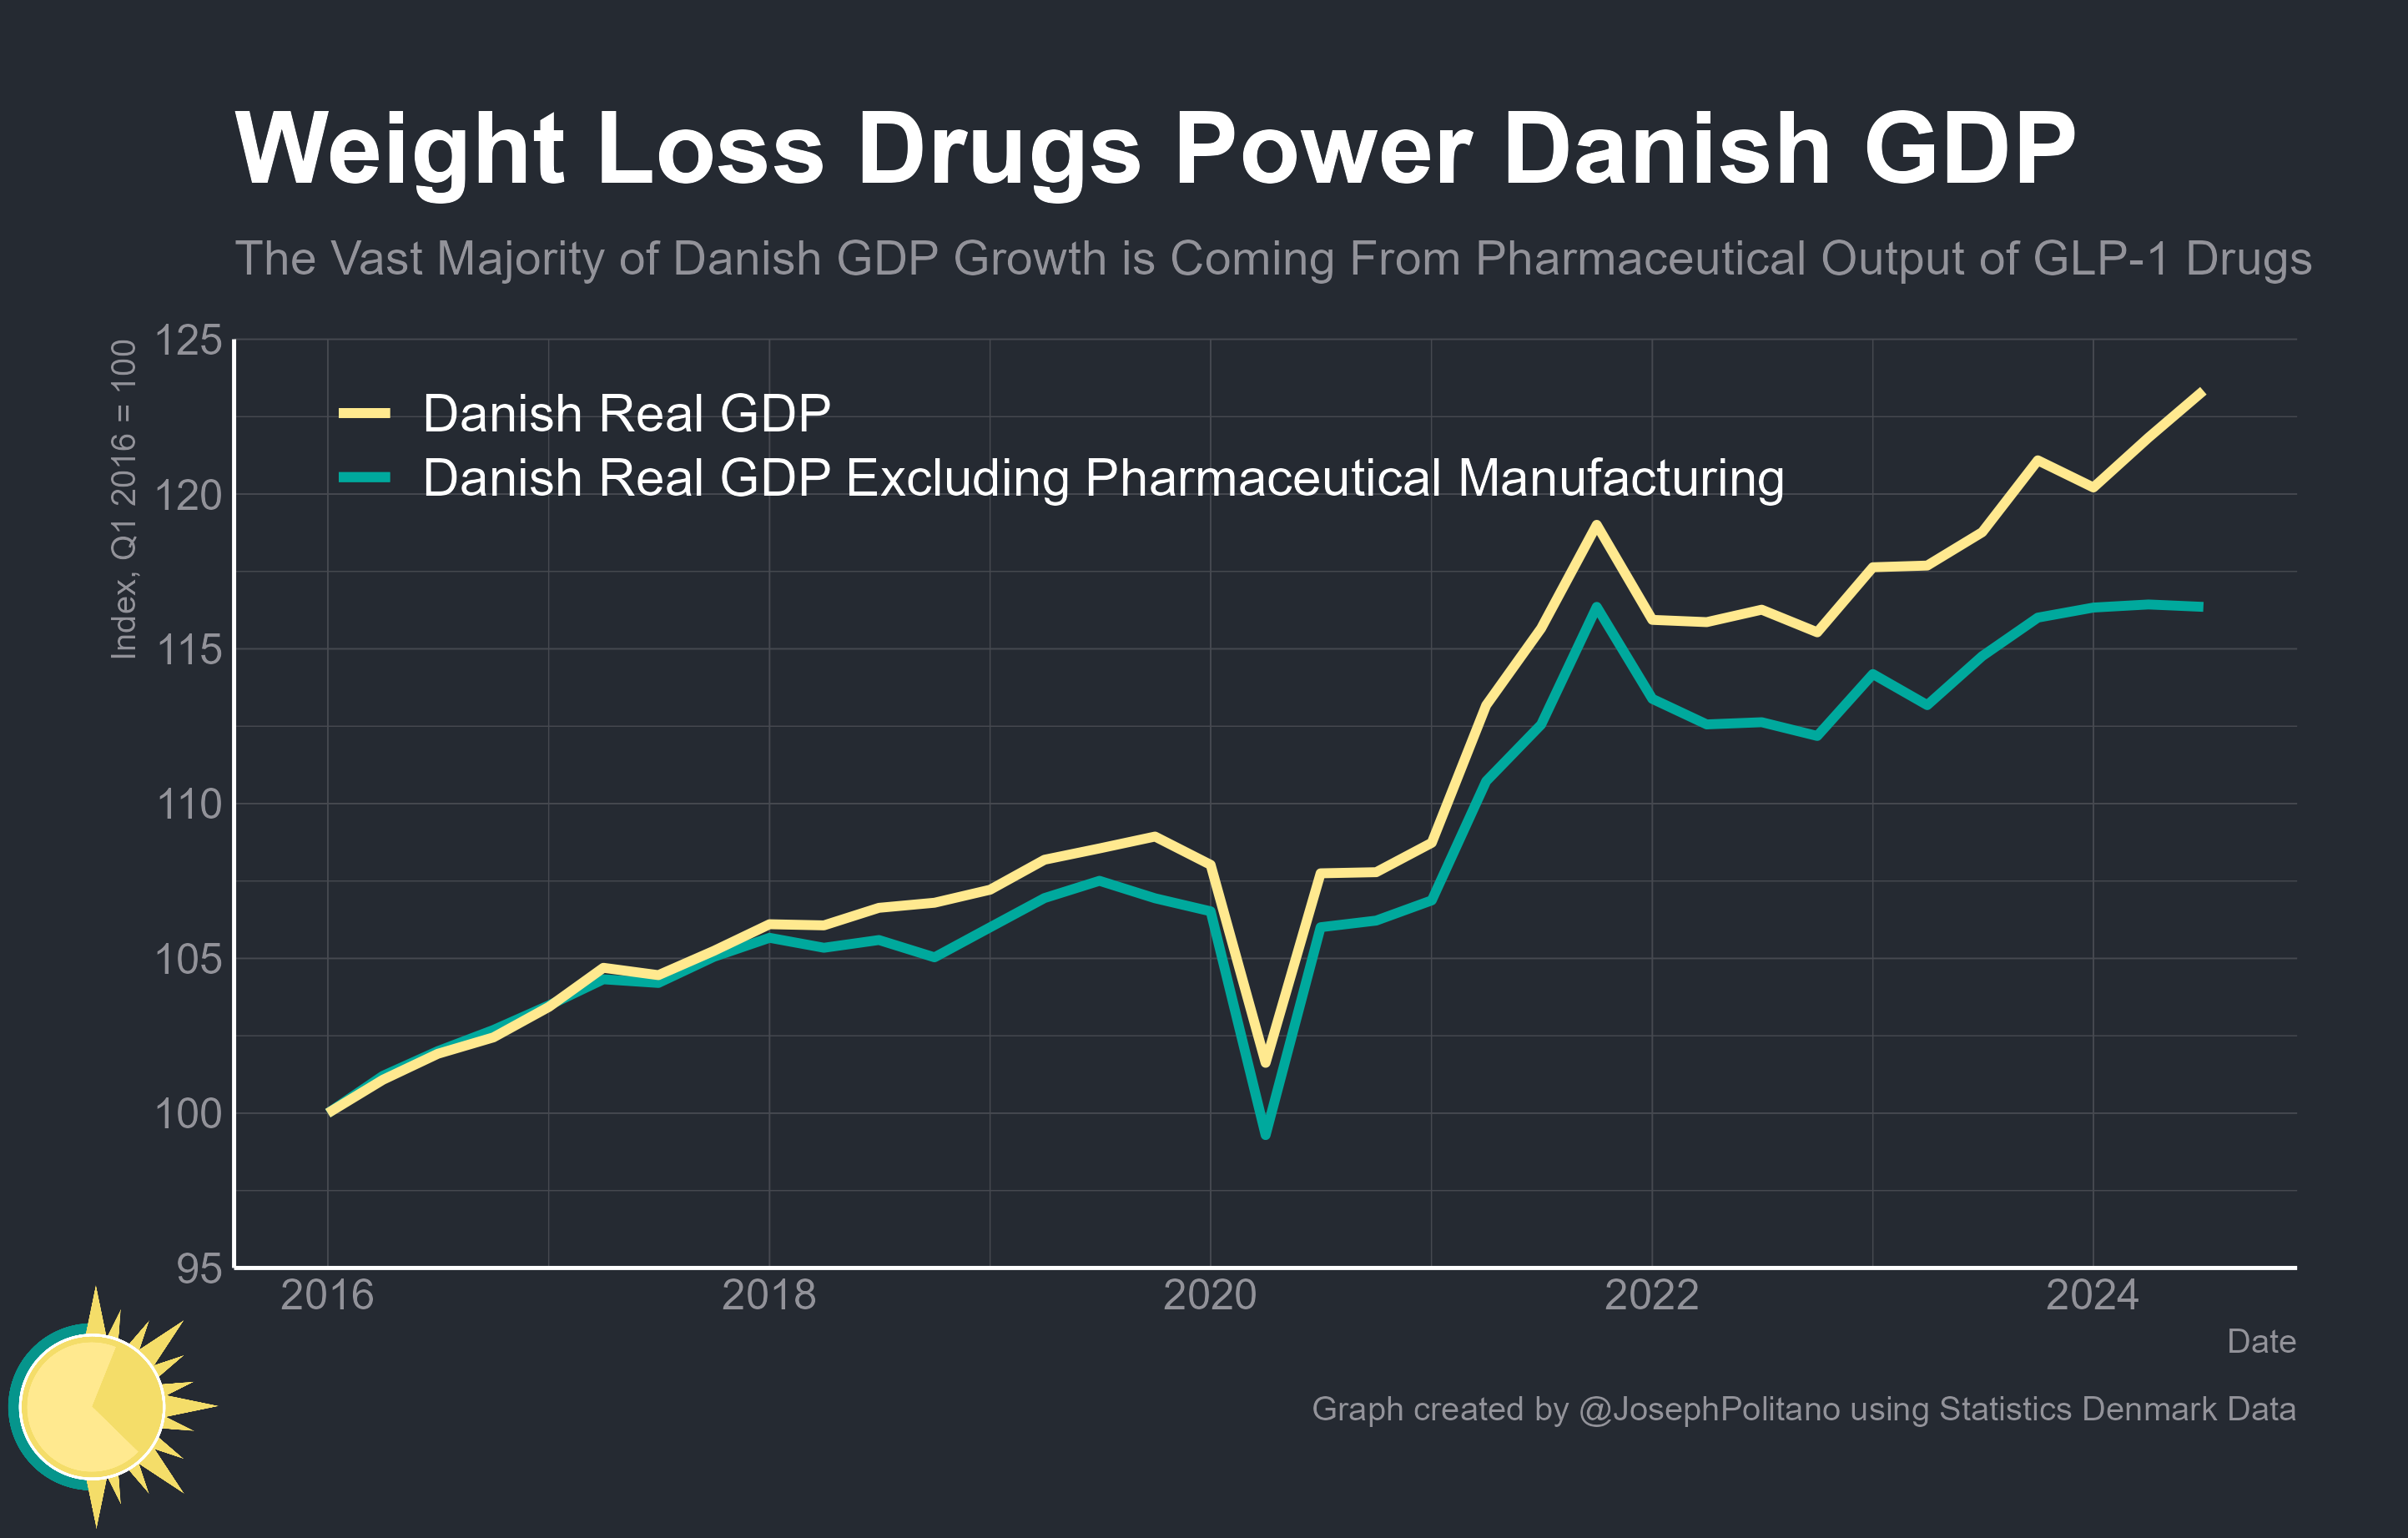
\includegraphics[width=0.8\linewidth]{figs/e081761e-ec32-4ea4-b1c8-e051139c24bf_2886x1843.png}
\end{figure}


\end{frame}


\begin{frame}{Production and Cost}
\Large Let us understand the mathematics of increasing returns.
\normalsize
\begin{wideitemize}
    \item Production function: $\underbrace{Y}_{\text{output}} = \underbrace{\ell^\alpha}_{\text{labor}}$ ($Y$ units produced when using $\ell$ labor) \\ $\implies \ell = Y^{\frac{1}{\alpha}}$ ($\ell$ required to produce $Y$ units)
    \onslide<2->{
    \item Fixed cost: $\bar{f}$
    }
    \onslide<3->{
    \item Cost function: $C(Y) = w \ell +\bar{f}= w Y^{\frac{1}{\alpha}} + F$ 
    }
    \onslide<4->{
    \item Average cost: $\frac{C(Y)}{Y} = w Y^{\frac{1}{\alpha} - 1}  + \frac{\bar{f}}{Y} $ 
    }
    \onslide<5->{
    \item Profits per unit: $\frac{\pi}{Y} = \frac{P Y - C(Y)}{Y} = P - AC$ $\implies$ firms will produce output when $P \ge AC$.
    }
\end{wideitemize}


\end{frame}




\begin{frame}{Production and Cost}
\Large Let us understand the mathematics of increasing returns.
\normalsize
\begin{wideitemize}
    \item Average cost: $\frac{C(Y)}{Y} = w Y^{\frac{1}{\alpha} - 1}  + \frac{\bar{f}}{Y} = \begin{cases} \frac{\partial }{\partial Y} \frac{C(Y)}{Y} > 0, & \text{decreasing returns to scale} \\ \frac{\partial }{\partial Y} \frac{C(Y)}{Y} = 0, & \text{constant returns to scale} \\
    \frac{\partial }{\partial Y} \frac{C(Y)}{Y} < 0, & \text{increasing returns to scale} \\
\end{cases}$ 

\end{wideitemize}


\end{frame}

\begin{frame}{Fixed costs and increasing returns}
\Large Constant, \textcolor{green}{increasing}, and \textcolor{red}{decreasing} returns to scale
\normalsize


    \onslide<2->{
    \centering
    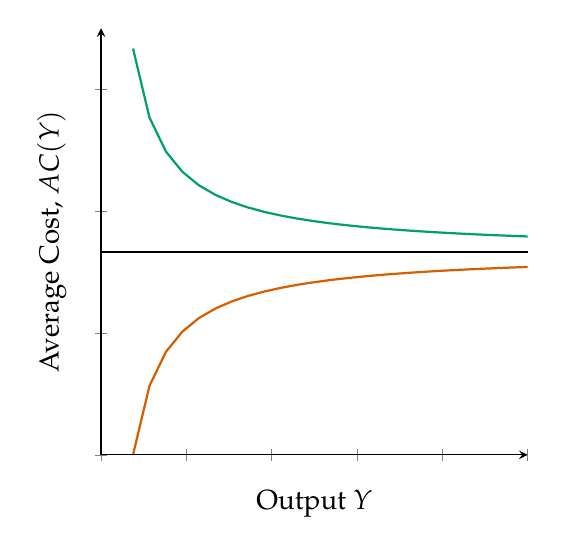
\begin{tikzpicture}
    \pgfmathsetmacro{\m}{0.3}
    \pgfmathsetmacro{\f}{2.5}

    
    
    \begin{axis}[
        ylabel={Average Cost, $AC(Y)$},
        xlabel={Output $Y$},        ymin=0, ymax=7,
        xmin=0, xmax=10,
        yticklabel=\empty,
        xticklabel=\empty,
        axis lines=left,
        enlargelimits=false,
        clip=false,
        axis on top,
        scaled x ticks=false,
        width=7cm, height=7cm,
        title style={font=\bfseries}
    ]

        \addplot[green, thick, domain=0.75:10] {1/\m + \f / x};
        \addplot[red, thick, domain=0.75:10] {1/\m  - \f / x};
        \addplot[black, thick, domain=0:10] {1/\m};

    \end{axis}

\end{tikzpicture}

}
\end{frame}



\begin{frame}{Production, Average Cost, and Increasing Returns to Scale}
\normalsize
\begin{wideitemize}
    \item Suppose production is $Y=\ell$ and fixed cost is $\bar{f}$
    
    \onslide<2->{
    \item If $\bar{f}=0$, then $C(Y) = wY$ and $AC(Y) = w$
    }
    \onslide<3->{
    \item if $\bar{f}>0$, then:
    }
    \onslide<4->{
    \begin{equation*}
    Y =
        \begin{cases}
            0 & \text{when } C(Y) \le\bar{f}\implies AC(Y) = \infty \\ 
            \ell & \text{when } C(Y) >\bar{f}\implies AC(Y) = w + \frac{\bar{f}}{Y}
            
        \end{cases}
        \end{equation*}
    }
    \onslide<5->{
    \item When $F>0$ and $C(Y) > F$, $AC(Y)$ is decreasing in Y $\implies$ increasing returns to scale!
    }
\end{wideitemize}


\end{frame}

\begin{frame}{Let us go back to our numerical example}
\Large Consider the production of a \textbf{new drug}.
\normalsize
\begin{wideitemize}
    \item to first to up with the medicine, there is a large \textbf{fixed cost investment} $\bar{f}$ of \$2.5 billion to develop and get approval for the drug 
    \onslide<2->{
    \item \textbf{Fixed Cost}: $\bar{f} = \$2.5 \text{billion}$
    }
    \onslide<3->{
    \item after the drug is developed and approved, producing new doses can be produced with a constant marginal cost: each 100 doses cost \$10 to produce
    }
    \onslide<4->{    
    \item \textbf{Variable cost}: \$0.1 
    \item \textbf{Total Cost}: $C(Y) = \$ 2.5 \text{billion} + \$ 0.1 Y $ 
    \item \textbf{Production}: $ Y = \begin{cases}
                                     0 & \text{if } C(Y) < \$ 2.5 \text{billion} \\
                                     \ell = (C-\$2.5B)/(\$0.1)  & \text{if } C(Y) \ge \$ 2.5 \text{billion} \\
                                    \end{cases}$
    }
\end{wideitemize}



\end{frame}

\begin{frame}{Total Cost}
\centering
\begin{columns}[T] % align columns
\begin{column}{.6\textwidth}
  \makebox[\linewidth][c]{
    \resizebox{\linewidth}{!}{
\centering
    \begin{tikzpicture}
    \pgfmathsetmacro{\m}{1}
    \pgfmathsetmacro{\f}{2.5}

    
    
    \begin{axis}[
        ylabel={$C(Y) = 1/10Y + \bar{f}$},
        xlabel={Output $Y$},
        ymin=0, ymax=10,
        xmin=0, xmax=10,
        yticklabel=\empty,
        xticklabel=\empty,
        axis lines=left,
        enlargelimits=false,
        clip=false,
        axis on top,
        scaled x ticks=false,
        width=7cm, height=6cm,
        title style={font=\bfseries}
    ]

        \addplot[green, thick, domain=0:7] {1/\m * x + \f};

        \node[anchor=east] at (axis cs:0,2.5) {$\bar{f}$};

    \end{axis}

\end{tikzpicture}
}
    }
\end{column}%
\hfill%
\begin{column}{.4\textwidth}
\begin{table}[]
\begin{tabular}{
>{\columncolor[HTML]{C6D9F1}}l>{\columncolor[HTML]{C6D9F1}}l}
\cellcolor[HTML]{4F81BD}Output (Million) & \cellcolor[HTML]{4F81BD}TC (Million) \\

500              & 2550         \\
1000             & 2600         \\
1500             & 2650         \\
2000             & 2700         \\
2500             & 2750         \\
3000             & 2800         \\
3500             & 2850        
\end{tabular}
\end{table}
\end{column}%
\end{columns}



\end{frame}

\begin{frame}{Average Cost}
\centering
\begin{columns}[T] % align columns
\begin{column}{.6\textwidth}
  \makebox[\linewidth][c]{
    \resizebox{\linewidth}{!}{
\centering
    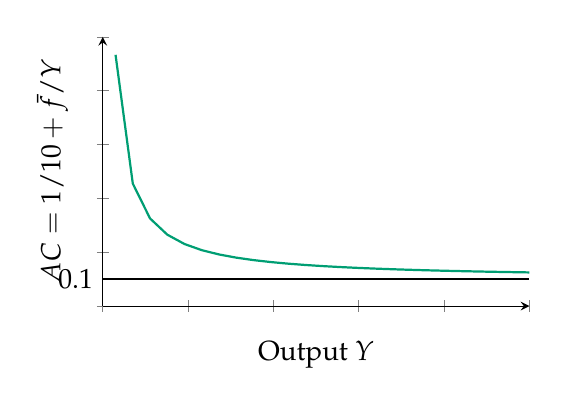
\begin{tikzpicture}
    \pgfmathsetmacro{\m}{1}
    \pgfmathsetmacro{\f}{2.5}

    
    
    \begin{axis}[
        ylabel={$AC = 1/10 + \bar{f}/Y$},
        xlabel={Output $Y$},
        ymin=0, ymax=10,
        xmin=0, xmax=10,
        yticklabel=\empty,
        xticklabel=\empty,
        axis lines=left,
        enlargelimits=false,
        clip=false,
        axis on top,
        scaled x ticks=false,
        width=7cm, height=5cm,
        title style={font=\bfseries}
    ]

        \addplot[green, thick, domain=0.3:10] {1/\m + \f / x};
        \addplot[black, thick, domain=0:10] {1/\m};
        \node[anchor=east] at (axis cs:0,1/\m) {$0.1$};

    \end{axis}

\end{tikzpicture}
}
    }
\end{column}%
\hfill%
\begin{column}{.4\textwidth}
\begin{table}[]
\begin{tabular}{
>{\columncolor[HTML]{C6D9F1}}l>{\columncolor[HTML]{C6D9F1}}l}
\cellcolor[HTML]{4F81BD}Output (Million) & \cellcolor[HTML]{4F81BD}AC (\$ per unit) \\
500              & 5.1          \\
1000             & 2.6          \\
1500             & 1.7          \\
2000             & 1.3          \\
2500             & 1.1          \\
3000             & 0.9          \\
3500             & 0.8         \\
\to \infty             & \to 0.1
\end{tabular}
\end{table}
\end{column}%
\end{columns}
\end{frame}

\begin{frame}{Inefficiency in Markets with Increasing Returns}
\centering

\centering
    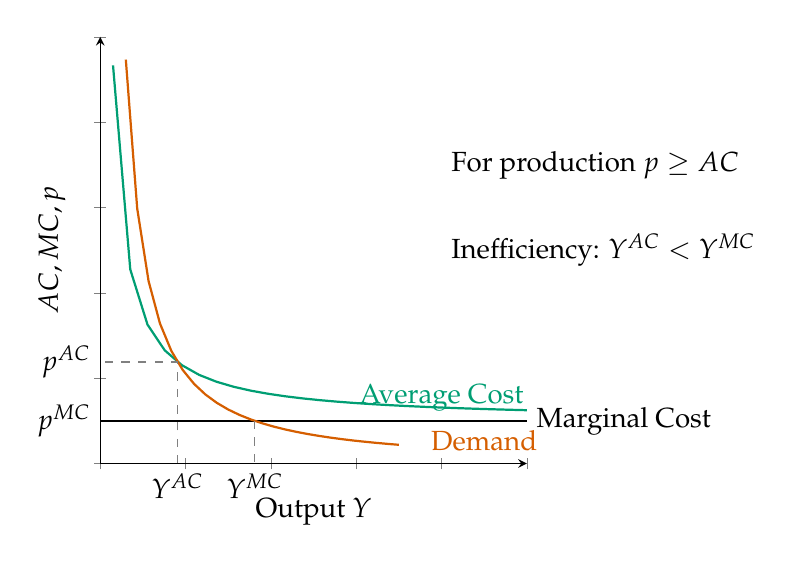
\begin{tikzpicture}
    \pgfmathsetmacro{\m}{1}
    \pgfmathsetmacro{\f}{2.5}
    \pgfmathsetmacro{\sigma}{1.25}

    
    
    \begin{axis}[
        ylabel={$AC, MC, p$},
        xlabel={Output $Y$},
        ymin=0, ymax=10,
        xmin=0, xmax=10,
        yticklabel=\empty,
        xticklabel=\empty,
        axis lines=left,
        enlargelimits=false,
        clip=false,
        axis on top,
        scaled x ticks=false,
        width=7cm, height=7cm,
        title style={font=\bfseries}
    ]

        \addplot[green, thick, domain=0.3:10] {1/\m + \f / x};
        \addplot[black, thick, domain=0:10] {1/\m};
        \addplot[red, thick, domain=0.6
        :7] {x^(-\sigma)*5};
        
         \addplot[gray, dashed] coordinates {(1.810454721,0) (1.810454721,{1/\m + \f / 1.810454721}) (0,{1/\m + \f / 1.810454721})};

        \addplot[gray, dashed] coordinates {((1/(5*\m))^(-1/\sigma) ,1/\m) ((1/(5*\m))^(-1/\sigma) ,0)};
        \node[anchor=north]at (axis cs:{(1/(5*\m))^(-1/\sigma)},0) {$Y^{MC}$};

        \node[anchor=south] at (axis cs: 8,{1/\m}) {\textcolor{green}{Average Cost}};

        \node[anchor=west] at (axis cs: 8,7) {For production $p \ge AC$};
        \node[anchor=west] at (axis cs: 8,5) {Inefficiency: $Y^{AC}<Y^{MC}$};

        \node[anchor=north]at (axis cs: 9,{1/\m}) {\textcolor{red}{Demand}};
 
        \node[anchor=west]at (axis cs: 10,{1/\m}) {Marginal Cost};
        \node[anchor=north] at (axis cs:{1.810454721,0 }) {$Y^{AC}$};

        \node[anchor=east] at (axis cs:{0,1/\m + \f / 1.810454721 }) {$p^{AC}$};

        \node[anchor=east] at (axis cs:0,1/\m) {$p^{MC}$};

    \end{axis}
    \end{tikzpicture}

\end{frame}


\begin{frame}
\Huge Micro diversion
\end{frame}

\begin{frame}{Problems with Perfect Competition}
\Large If price is equal to marginal cost, no firm will undertake the costly research that is
necessary to invent new ideas.
\vspace{20pt}

\normalsize

\begin{wideitemize}
    \item Wedge between $P$ and $MC$ to remunerate innovators (e.g.: Patents assign monopoly power for 20 years to innovators)
    \item  $P > MC$ (market power) has negative consequences: people priced out of market, lower overall surplus
\end{wideitemize}
    
\end{frame}


  \begin{frame}{Supply in a Competitive Market}
  \begin{columns}[T] % align columns
\begin{column}{.4\textwidth}
\Large Firm \textbf{takes prices as given} and chooses labor to maximize profits
\normalsize
\begin{equation*}
    \max_{\{Y\}} \pi = PY - C(Y)
\end{equation*}

Solution for optimal $C$:
\begin{equation*}
    P = C'(Y) = MC
\end{equation*}


\end{column}%
\hfill%
\begin{column}{.6\textwidth}
  \makebox[\linewidth][c]{
    \resizebox{\linewidth}{!}{

\centering
    \begin{tikzpicture}
    \pgfmathsetmacro{\m}{1}
    \pgfmathsetmacro{\f}{2.5}
    \pgfmathsetmacro{\sigma}{1.25}

    
    
    \begin{axis}[
        ylabel={$AC, MC, p$},
        xlabel={Output $Y$},
        ymin=0, ymax=10,
        xmin=0, xmax=10,
        yticklabel=\empty,
        xticklabel=\empty,
        axis lines=left,
        enlargelimits=false,
        clip=false,
        axis on top,
        scaled x ticks=false,
        width=7cm, height=7cm,
        title style={font=\bfseries}
    ]

        \addplot[black, thick, domain=0:10] {1/\m};

        \node[anchor=west] at (axis cs: 8,7) {Infinitely elastic supply};

 
        \node[anchor=west]at (axis cs: 10,{1/\m}) {Marginal Cost};


        \node[anchor=east] at (axis cs:0,1/\m) {$p^{MC}$};

    \end{axis}
    \end{tikzpicture}

      }
    }

\end{column}%
\end{columns}
\end{frame}


\begin{frame}{Logic of a monopolist}

  \begin{wideitemize}
      \item Take (inverse) demand curve $P(Y)$ as given and choose supply that maximizes profits
      \begin{equation*}
        \max_{\{Y\}} \pi = P(Y) Y - C(Y) 
    \end{equation*}


      \item Optimal choice:

      \begin{equation*}
          MR = P(Y) + P'(Y)Y = C'(Y) = MC
      \end{equation*}

      \item To sell incremental unit, firm must lower price for all units \\
      \qquad (including inframarginal units)

      \item Suppose $P(Y) = (A/b) - (1/b)Y$, then:

      \begin{equation*}
          P(Y) + P'(Y)Y= (A/b) - (1/b)Y - (1/b)Y = (A/b) - (2/b)Y 
      \end{equation*}

      
  \end{wideitemize}

  
\end{frame}


\section{Monopoly}

\begin{frame}{Market Structures}

\begin{wideitemize}
    \item Monopoly: One firms serves the entire market
    \item Oligopoly (duopoly): Several (two) firms serve the market and compete partially, each anticipating each others’ rational actions
    \item Monopolistic competition: No reaction to other firms’ supply
    \begin{itemize}
        \item Products differentiated from competitors.
        \item One firm per niche market
        \item Competitors’ supply (price choice) taken as given
    \end{itemize}

\end{wideitemize}

\end{frame}


\begin{frame}{Monopoly}
\centering
    \begin{tikzpicture}
    \pgfmathsetmacro{\A}{7}
    \pgfmathsetmacro{\b}{0.75}
    \pgfmathsetmacro{\m}{0.35}
    \pgfmathsetmacro{\pmax}{\A/\b}          % choke price  (demand intercept)
    \pgfmathsetmacro{\qc}{\A - \b/\m}       % competitive quantity (P = MC)
        
    
    
    \begin{axis}[
        xlabel={Output $Y$},
        ymin=0, ymax=10,
        xmin=0, xmax=5,
        yticklabel=\empty,
        xticklabel=\empty,
        axis lines=left,
        enlargelimits=false,
        clip=false,
        axis on top,
        scaled x ticks=false,
        width=7cm, height=7cm,
        title style={font=\bfseries}
    ]

        \pgfmathsetmacro{\q}{((\A / \b - 1/ \m ) / ( 2/\b))}
        \pgfmathsetmacro{\p}{ (\A / \b) - 1/\b * \q }
        \pgfmathsetmacro{\pc}{ (\A / \b) - 2/\b * \q }
                    
        \addplot[purple, thick, domain=0:5] {(\A / \b) - 1/\b * x};
        %\pgfmathsetmacro{\f}{\p * \q - \q / \m}
        %\addplot[blue, thick, domain=1:5] {1/\m + \f / x};

        
        \pgfmathsetmacro{\d}{ -.75 }
        \pgfmathsetmacro{\qd}{ \q+\d }
        \pgfmathsetmacro{\pd}{ (\A / \b) - 1/\b * (\qd) }

        \addplot[gray, dashed] coordinates {(\q,\p) (\qd,\p) (\qd,\pd)};
        \node[anchor=north] at (axis cs: {\qd + (\q-\qd)/2},\p) {$1$};
        \node[anchor=east] at (axis cs: \qd,{\pd - (\pd-\p)/2}) {$\frac{1}{b}$};



        %\node[anchor=south west] at (axis cs: 5,{1/\m+.43}) {\textcolor{blue}{Average Cost}};
        \node[anchor=west] at (axis cs: 3,\p) {\scriptsize \textcolor{purple}{Demand}};


    \end{axis}

    \end{tikzpicture}

 \end{frame}


\begin{frame}{Monopoly}
\addtocounter{framenumber}{-1}
\centering
    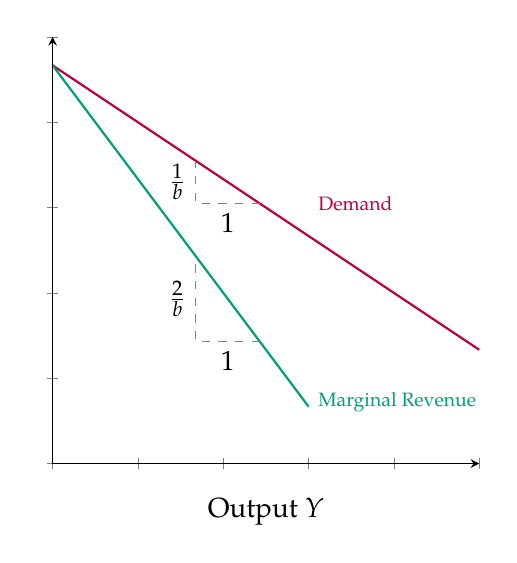
\begin{tikzpicture}
    \pgfmathsetmacro{\A}{7}
    \pgfmathsetmacro{\b}{0.75}
    \pgfmathsetmacro{\m}{0.35}
    \pgfmathsetmacro{\pmax}{\A/\b}          % choke price  (demand intercept)
    \pgfmathsetmacro{\qc}{\A - \b/\m}       % competitive quantity (P = MC)
        
    
    
    \begin{axis}[
        xlabel={Output $Y$},
        ymin=0, ymax=10,
        xmin=0, xmax=5,
        yticklabel=\empty,
        xticklabel=\empty,
        axis lines=left,
        enlargelimits=false,
        clip=false,
        axis on top,
        scaled x ticks=false,
        width=7cm, height=7cm,
        title style={font=\bfseries}
    ]

        \pgfmathsetmacro{\q}{((\A / \b - 1/ \m ) / ( 2/\b))}
        \pgfmathsetmacro{\p}{ (\A / \b) - 1/\b * \q }
        \pgfmathsetmacro{\pc}{ (\A / \b) - 2/\b * \q }
                    
        \addplot[purple, thick, domain=0:5] {(\A / \b) - 1/\b * x};
        \addplot[green, thick, domain=0:3] {(\A / \b) - 2/\b * x};
        %\pgfmathsetmacro{\f}{\p * \q - \q / \m}
        %\addplot[blue, thick, domain=1:5] {1/\m + \f / x};

        
        \pgfmathsetmacro{\d}{ -.75 }
        \pgfmathsetmacro{\qd}{ \q+\d }
        \pgfmathsetmacro{\pd}{ (\A / \b) - 1/\b * (\qd) }

        \addplot[gray, dashed] coordinates {(\q,\p) (\qd,\p) (\qd,\pd)};
        \node[anchor=north] at (axis cs: {\qd + (\q-\qd)/2},\p) {$1$};
        \node[anchor=east] at (axis cs: \qd,{\pd - (\pd-\p)/2}) {$\frac{1}{b}$};


        \pgfmathsetmacro{\pcd}{ (\A / \b) - 2/\b * (\qd) }

        \addplot[gray, dashed] coordinates {(\q,\pc) (\qd,\pc) (\qd,\pcd)};
        \node[anchor=north] at (axis cs: {\qd + (\q-\qd)/2},\pc) {$1$};
        \node[anchor=east] at (axis cs: \qd,{\pcd - (\pcd-\pc)/2}) {$\frac{2}{b}$};
        %\addplot[gray, dashed] coordinates {(\q,1/\m + \f / \q) (0,1/\m + \f / \q)};
        %\addplot[only marks, mark=*, color=black, mark size=2pt] coordinates {(\q,1/\m + \f / \q)};

        %\node[anchor=south west] at (axis cs: 5,{1/\m+.43}) {\textcolor{blue}{Average Cost}};
        \node[anchor=west] at (axis cs: 3,\p) {\scriptsize \textcolor{purple}{Demand}};
        \node[anchor=west] at (axis cs: 3,{1/(2*\m)}) {\textcolor{green}{\scriptsize Marginal Revenue}};



    \end{axis}

    \end{tikzpicture}

 \end{frame}


\begin{frame}{Monopoly}
\addtocounter{framenumber}{-1}
\centering
    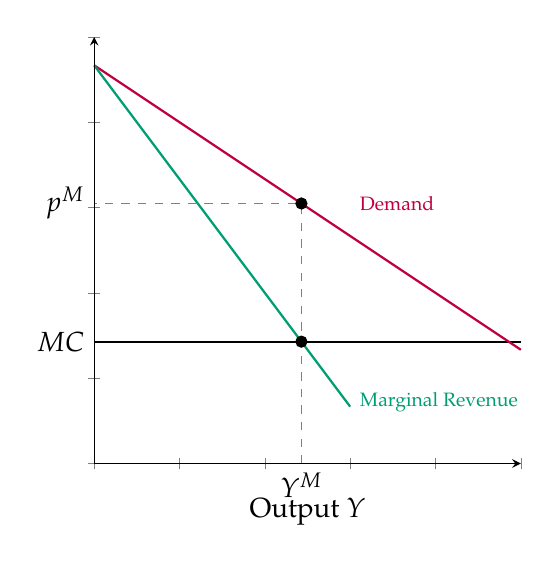
\begin{tikzpicture}
    \pgfmathsetmacro{\A}{7}
    \pgfmathsetmacro{\b}{0.75}
    \pgfmathsetmacro{\m}{0.35}
    \pgfmathsetmacro{\pmax}{\A/\b}          % choke price  (demand intercept)
    \pgfmathsetmacro{\qc}{\A - \b/\m}       % competitive quantity (P = MC)
        
    
    
    \begin{axis}[
        xlabel={Output $Y$},
        ymin=0, ymax=10,
        xmin=0, xmax=5,
        yticklabel=\empty,
        xticklabel=\empty,
        axis lines=left,
        enlargelimits=false,
        clip=false,
        axis on top,
        scaled x ticks=false,
        width=7cm, height=7cm,
        title style={font=\bfseries}
    ]

        \pgfmathsetmacro{\q}{((\A / \b - 1/ \m ) / ( 2/\b))}
        \pgfmathsetmacro{\p}{ (\A / \b) - 1/\b * \q }
                    
        \addplot[black, thick, domain=0:5] {1/\m};
        \addplot[purple, thick, domain=0:5] {(\A / \b) - 1/\b * x};
        \addplot[green, thick, domain=0:3] {(\A / \b) - 2/\b * x};
        %\pgfmathsetmacro{\f}{\p * \q - \q / \m}
        %\addplot[blue, thick, domain=1:5] {1/\m + \f / x};

        
        \addplot[gray, dashed] coordinates {(\q,0) (\q,\p) (0,\p)};
        \addplot[only marks, mark=*, color=black, mark size=2pt] coordinates {(\q,\p)};
        \addplot[only marks, mark=*, color=black, mark size=2pt] coordinates {(\q,1/\m)};

        %\addplot[gray, dashed] coordinates {(\q,1/\m + \f / \q) (0,1/\m + \f / \q)};
        %\addplot[only marks, mark=*, color=black, mark size=2pt] coordinates {(\q,1/\m + \f / \q)};

        %\node[anchor=south west] at (axis cs: 5,{1/\m+.43}) {\textcolor{blue}{Average Cost}};
        \node[anchor=west] at (axis cs: 3,\p) {\scriptsize \textcolor{purple}{Demand}};
        \node[anchor=west] at (axis cs: 3,{1/(2*\m)}) {\textcolor{green}{\scriptsize Marginal Revenue}};

        \node[anchor=east] at (axis cs: 0,\p) {$p^{M}$};
        \node[anchor=east] at (axis cs: 0,1/ \m) {$MC$};

        \node[anchor=north] at (axis cs: \q,0) {$Y^{M}$};

    \end{axis}

    \end{tikzpicture}

 \end{frame}



\begin{frame}{Monopoly}
\addtocounter{framenumber}{-1}
\centering
    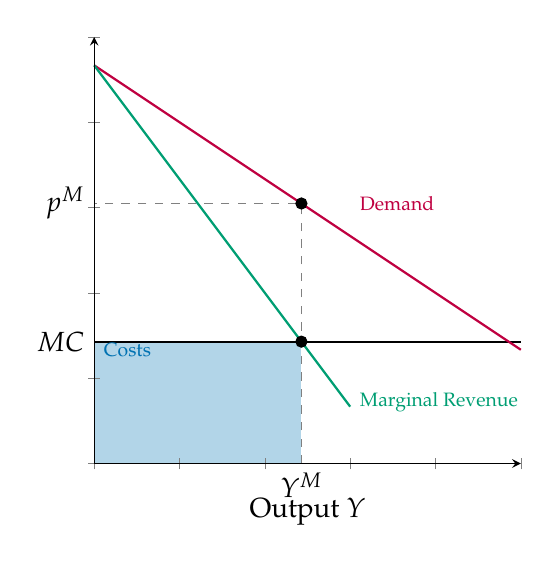
\begin{tikzpicture}
    \pgfmathsetmacro{\A}{7}
    \pgfmathsetmacro{\b}{0.75}
    \pgfmathsetmacro{\m}{0.35}
    \pgfmathsetmacro{\pmax}{\A/\b}          % choke price  (demand intercept)
    \pgfmathsetmacro{\qc}{\A - \b/\m}       % competitive quantity (P = MC)
        
    
    
    \begin{axis}[
        xlabel={Output $Y$},
        ymin=0, ymax=10,
        xmin=0, xmax=5,
        yticklabel=\empty,
        xticklabel=\empty,
        axis lines=left,
        enlargelimits=false,
        clip=false,
        axis on top,
        scaled x ticks=false,
        width=7cm, height=7cm,
        title style={font=\bfseries}
    ]

        \pgfmathsetmacro{\q}{((\A / \b - 1/ \m ) / ( 2/\b))}
        \pgfmathsetmacro{\p}{ (\A / \b) - 1/\b * \q }
        % costs
        \addplot[fill=blue!30, draw=none] coordinates
            {(0,0) (0,1/\m) (\q,1/\m) (\q,0)} -- cycle;
                    
        \addplot[black, thick, domain=0:5] {1/\m};
        \addplot[purple, thick, domain=0:5] {(\A / \b) - 1/\b * x};
        \addplot[green, thick, domain=0:3] {(\A / \b) - 2/\b * x};
        %\pgfmathsetmacro{\f}{\p * \q - \q / \m}
        %\addplot[blue, thick, domain=1:5] {1/\m + \f / x};

        
        \addplot[gray, dashed] coordinates {(\q,0) (\q,\p) (0,\p)};
        \addplot[only marks, mark=*, color=black, mark size=2pt] coordinates {(\q,\p)};
        \addplot[only marks, mark=*, color=black, mark size=2pt] coordinates {(\q,1/\m)};

        %\addplot[gray, dashed] coordinates {(\q,1/\m + \f / \q) (0,1/\m + \f / \q)};
        %\addplot[only marks, mark=*, color=black, mark size=2pt] coordinates {(\q,1/\m + \f / \q)};

        \node[anchor = north west] at (axis cs: 0,{1/(\m)+.2}) {\scriptsize \textcolor{blue}{Costs}};

        %\node[anchor=south west] at (axis cs: 5,{1/\m+.43}) {\textcolor{blue}{Average Cost}};
        \node[anchor=west] at (axis cs: 3,\p) {\scriptsize \textcolor{purple}{Demand}};
        \node[anchor=west] at (axis cs: 3,{1/(2*\m)}) {\textcolor{green}{\scriptsize Marginal Revenue}};

        \node[anchor=east] at (axis cs: 0,\p) {$p^{M}$};
        \node[anchor=east] at (axis cs: 0,1/ \m) {$MC$};

        \node[anchor=north] at (axis cs: \q,0) {$Y^{M}$};

    \end{axis}

    \end{tikzpicture}

 \end{frame}




\begin{frame}{Monopoly}
\addtocounter{framenumber}{-1}
\centering
    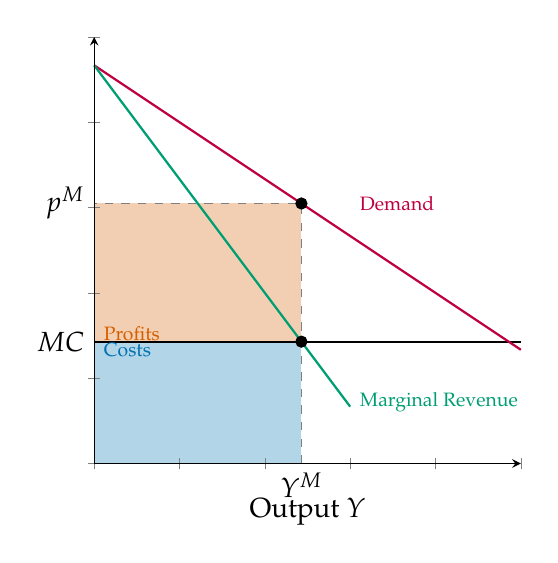
\begin{tikzpicture}
    \pgfmathsetmacro{\A}{7}
    \pgfmathsetmacro{\b}{0.75}
    \pgfmathsetmacro{\m}{0.35}
    \pgfmathsetmacro{\pmax}{\A/\b}          % choke price  (demand intercept)
    \pgfmathsetmacro{\qc}{\A - \b/\m}       % competitive quantity (P = MC)
        
    
    
    \begin{axis}[
        xlabel={Output $Y$},
        ymin=0, ymax=10,
        xmin=0, xmax=5,
        yticklabel=\empty,
        xticklabel=\empty,
        axis lines=left,
        enlargelimits=false,
        clip=false,
        axis on top,
        scaled x ticks=false,
        width=7cm, height=7cm,
        title style={font=\bfseries}
    ]

        \pgfmathsetmacro{\q}{((\A / \b - 1/ \m ) / ( 2/\b))}
        \pgfmathsetmacro{\p}{ (\A / \b) - 1/\b * \q }
        % profits
        \addplot[fill=red!30, draw=none] coordinates
            {(0,1/\m) (0,\p) (\q,\p) (\q,1/\m)} -- cycle;
        % costs
        \addplot[fill=blue!30, draw=none] coordinates
            {(0,0) (0,1/\m) (\q,1/\m) (\q,0)} -- cycle;
                    
        \addplot[black, thick, domain=0:5] {1/\m};
        \addplot[purple, thick, domain=0:5] {(\A / \b) - 1/\b * x};
        \addplot[green, thick, domain=0:3] {(\A / \b) - 2/\b * x};
        %\pgfmathsetmacro{\f}{\p * \q - \q / \m}
        %\addplot[blue, thick, domain=1:5] {1/\m + \f / x};

        
        \addplot[gray, dashed] coordinates {(\q,0) (\q,\p) (0,\p)};
        \addplot[only marks, mark=*, color=black, mark size=2pt] coordinates {(\q,\p)};
        \addplot[only marks, mark=*, color=black, mark size=2pt] coordinates {(\q,1/\m)};

        %\addplot[gray, dashed] coordinates {(\q,1/\m + \f / \q) (0,1/\m + \f / \q)};
        %\addplot[only marks, mark=*, color=black, mark size=2pt] coordinates {(\q,1/\m + \f / \q)};

        \node[anchor = south west] at (axis cs: 0,{1/(\m)-.2}) {\scriptsize \textcolor{red}{Profits}};
        \node[anchor = north west] at (axis cs: 0,{1/(\m)+.2}) {\scriptsize \textcolor{blue}{Costs}};

        %\node[anchor=south west] at (axis cs: 5,{1/\m+.43}) {\textcolor{blue}{Average Cost}};
        \node[anchor=west] at (axis cs: 3,\p) {\scriptsize \textcolor{purple}{Demand}};
        \node[anchor=west] at (axis cs: 3,{1/(2*\m)}) {\textcolor{green}{\scriptsize Marginal Revenue}};

        \node[anchor=east] at (axis cs: 0,\p) {$p^{M}$};
        \node[anchor=east] at (axis cs: 0,1/ \m) {$MC$};

        \node[anchor=north] at (axis cs: \q,0) {$Y^{M}$};

    \end{axis}

    \end{tikzpicture}

 \end{frame}



\begin{frame}{Monopoly}
\addtocounter{framenumber}{-1}
\centering
    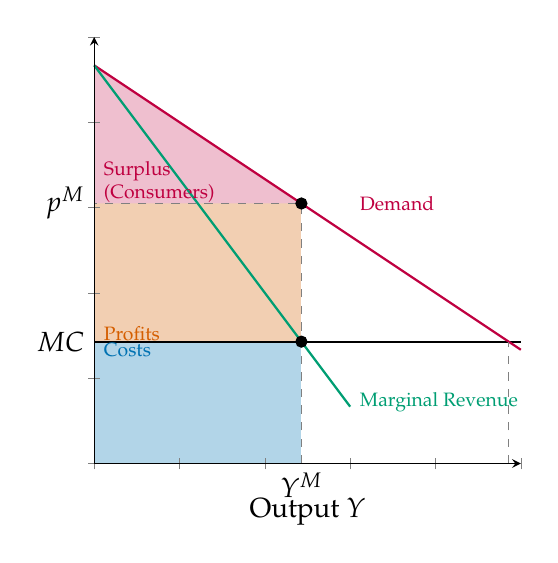
\begin{tikzpicture}
    \pgfmathsetmacro{\A}{7}
    \pgfmathsetmacro{\b}{0.75}
    \pgfmathsetmacro{\m}{0.35}
    \pgfmathsetmacro{\pmax}{\A/\b}          % choke price  (demand intercept)
    \pgfmathsetmacro{\qc}{\A - \b/\m}       % competitive quantity (P = MC)
        
    
    
    \begin{axis}[
        xlabel={Output $Y$},
        ymin=0, ymax=10,
        xmin=0, xmax=5,
        yticklabel=\empty,
        xticklabel=\empty,
        axis lines=left,
        enlargelimits=false,
        clip=false,
        axis on top,
        scaled x ticks=false,
        width=7cm, height=7cm,
        title style={font=\bfseries}
    ]

        \pgfmathsetmacro{\q}{((\A / \b - 1/ \m ) / ( 2/\b))}
        \pgfmathsetmacro{\p}{ (\A / \b) - 1/\b * \q }
        % profits
        \addplot[fill=red!30, draw=none] coordinates
            {(0,1/\m) (0,\p) (\q,\p) (\q,1/\m)} -- cycle;
        % costs
        \addplot[fill=blue!30, draw=none] coordinates
            {(0,0) (0,1/\m) (\q,1/\m) (\q,0)} -- cycle;
        % consumer-surplus
        \addplot[fill=purple!25, draw=none] coordinates
            {(0,\p) (0,\pmax) (\q,\p)} -- cycle;
                    
        \addplot[black, thick, domain=0:5] {1/\m};
        \addplot[purple, thick, domain=0:5] {(\A / \b) - 1/\b * x};
        \addplot[green, thick, domain=0:3] {(\A / \b) - 2/\b * x};
        %\pgfmathsetmacro{\f}{\p * \q - \q / \m}
        %\addplot[blue, thick, domain=1:5] {1/\m + \f / x};

        
        \addplot[gray, dashed] coordinates {(\q,0) (\q,\p) (0,\p)};
        \addplot[only marks, mark=*, color=black, mark size=2pt] coordinates {(\q,\p)};
        \addplot[only marks, mark=*, color=black, mark size=2pt] coordinates {(\q,1/\m)};
        \addplot[gray, dashed] coordinates {(\qc,0) (\qc,1/\m)};

        %\addplot[gray, dashed] coordinates {(\q,1/\m + \f / \q) (0,1/\m + \f / \q)};
        %\addplot[only marks, mark=*, color=black, mark size=2pt] coordinates {(\q,1/\m + \f / \q)};

        \node[anchor = south west] at (axis cs: 0,{\p+.3}) {\scriptsize \textcolor{purple}{Surplus}};
        \node[anchor = south west] at (axis cs: 0,{\p-.2}) {\scriptsize \textcolor{purple}{(Consumers)}};
        \node[anchor = south west] at (axis cs: 0,{1/(\m)-.2}) {\scriptsize \textcolor{red}{Profits}};
        \node[anchor = north west] at (axis cs: 0,{1/(\m)+.2}) {\scriptsize \textcolor{blue}{Costs}};

        %\node[anchor=south west] at (axis cs: 5,{1/\m+.43}) {\textcolor{blue}{Average Cost}};
        \node[anchor=west] at (axis cs: 3,\p) {\scriptsize \textcolor{purple}{Demand}};
        \node[anchor=west] at (axis cs: 3,{1/(2*\m)}) {\textcolor{green}{\scriptsize Marginal Revenue}};

        \node[anchor=east] at (axis cs: 0,\p) {$p^{M}$};
        \node[anchor=east] at (axis cs: 0,1/ \m) {$MC$};

        \node[anchor=north] at (axis cs: \q,0) {$Y^{M}$};

    \end{axis}

    \end{tikzpicture}

 \end{frame}

\begin{frame}{Monopoly}
\addtocounter{framenumber}{-1}
\centering
    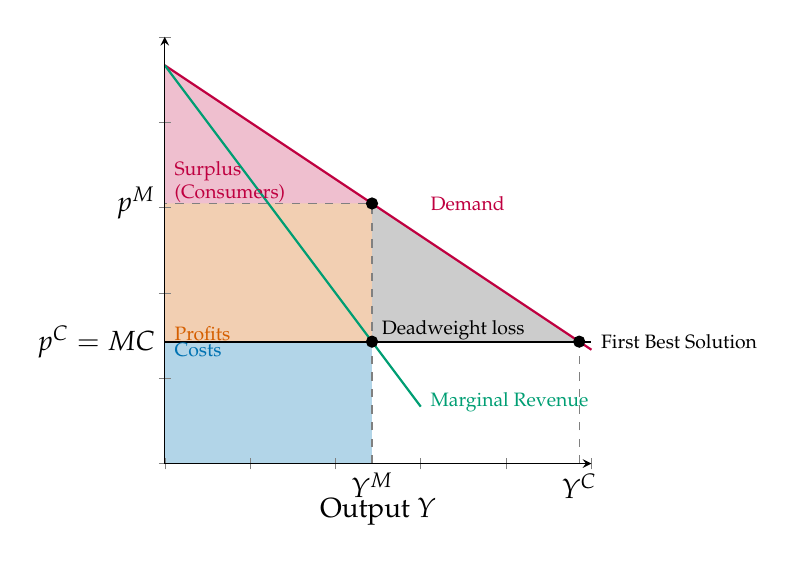
\begin{tikzpicture}
    \pgfmathsetmacro{\A}{7}
    \pgfmathsetmacro{\b}{0.75}
    \pgfmathsetmacro{\m}{0.35}
    \pgfmathsetmacro{\pmax}{\A/\b}          % choke price  (demand intercept)
    \pgfmathsetmacro{\qc}{\A - \b/\m}       % competitive quantity (P = MC)
        
    
    
    \begin{axis}[
        xlabel={Output $Y$},
        ymin=0, ymax=10,
        xmin=0, xmax=5,
        yticklabel=\empty,
        xticklabel=\empty,
        axis lines=left,
        enlargelimits=false,
        clip=false,
        axis on top,
        scaled x ticks=false,
        width=7cm, height=7cm,
        title style={font=\bfseries}
    ]

        \pgfmathsetmacro{\q}{((\A / \b - 1/ \m ) / ( 2/\b))}
        \pgfmathsetmacro{\p}{ (\A / \b) - 1/\b * \q }
        % profits
        \addplot[fill=red!30, draw=none] coordinates
            {(0,1/\m) (0,\p) (\q,\p) (\q,1/\m)} -- cycle;
        % costs
        \addplot[fill=blue!30, draw=none] coordinates
            {(0,0) (0,1/\m) (\q,1/\m) (\q,0)} -- cycle;
        % consumer-surplus
        \addplot[fill=purple!25, draw=none] coordinates
            {(0,\p) (0,\pmax) (\q,\p)} -- cycle;
        
        % deadweight loss
        \addplot[fill=gray!40, draw=none] coordinates
            {(\q,\p) (\qc,1/\m) (\q,1/\m)} -- cycle;
            
        \addplot[black, thick, domain=0:5] {1/\m};
        \addplot[purple, thick, domain=0:5] {(\A / \b) - 1/\b * x};
        \addplot[green, thick, domain=0:3] {(\A / \b) - 2/\b * x};
        %\pgfmathsetmacro{\f}{\p * \q - \q / \m}
        %\addplot[blue, thick, domain=1:5] {1/\m + \f / x};

        
        \addplot[gray, dashed] coordinates {(\q,0) (\q,\p) (0,\p)};
        \addplot[only marks, mark=*, color=black, mark size=2pt] coordinates {(\q,\p)};
        \addplot[only marks, mark=*, color=black, mark size=2pt] coordinates {(\q,1/\m)};
        \addplot[gray, dashed] coordinates {(\qc,0) (\qc,1/\m)};
        \addplot[only marks, mark=*, color=black, mark size=2pt] coordinates {(\qc,1/\m)};

        %\addplot[gray, dashed] coordinates {(\q,1/\m + \f / \q) (0,1/\m + \f / \q)};
        %\addplot[only marks, mark=*, color=black, mark size=2pt] coordinates {(\q,1/\m + \f / \q)};

        \node[anchor = south west] at (axis cs: 0,{\p+.3}) {\scriptsize \textcolor{purple}{Surplus}};
        \node[anchor = south west] at (axis cs: 0,{\p-.2}) {\scriptsize \textcolor{purple}{(Consumers)}};
        \node[anchor = south west] at (axis cs: 0,{1/(\m)-.2}) {\scriptsize \textcolor{red}{Profits}};
        \node[anchor = north west] at (axis cs: 0,{1/(\m)+.2}) {\scriptsize \textcolor{blue}{Costs}};
        \node[anchor = south west] at (axis cs: \q,{1/(\m)-.2}) {\scriptsize Deadweight loss};

        %\node[anchor=south west] at (axis cs: 5,{1/\m+.43}) {\textcolor{blue}{Average Cost}};
        \node[anchor=west] at (axis cs: 3,\p) {\scriptsize \textcolor{purple}{Demand}};
        \node[anchor=west] at (axis cs: 5,{1/\m}) {\scriptsize First Best Solution};
        \node[anchor=west] at (axis cs: 3,{1/(2*\m)}) {\textcolor{green}{\scriptsize Marginal Revenue}};

        \node[anchor=east] at (axis cs: 0,\p) {$p^{M}$};
        \node[anchor=east] at (axis cs: 0,1/ \m) {$p^{C}=MC$};

        \node[anchor=north] at (axis cs: \q,0) {$Y^{M}$};
        \node[anchor=north] at (axis cs: \qc,0) {$Y^{C}$};

    \end{axis}

    \end{tikzpicture}

 \end{frame}

 
\begin{frame}{What if marginal cost function are different? (decreasing returns)}
\addtocounter{framenumber}{-1}
\centering
    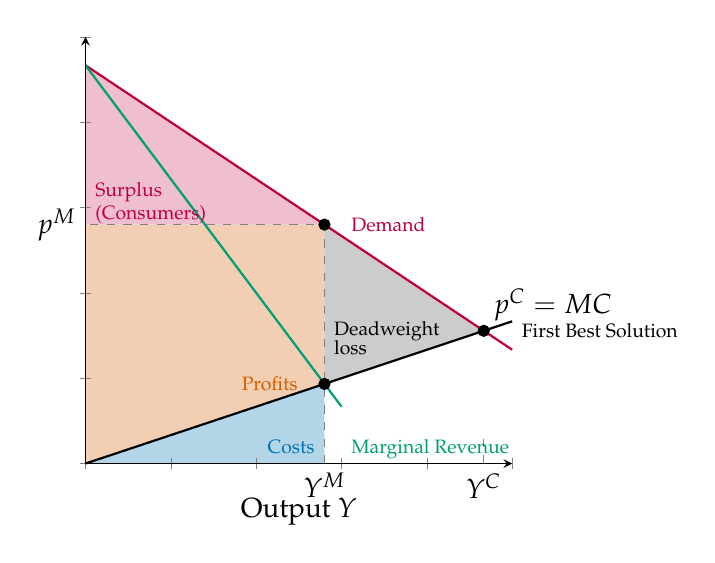
\begin{tikzpicture}
    \pgfmathsetmacro{\A}{7}
    \pgfmathsetmacro{\b}{0.75}
    \pgfmathsetmacro{\m}{1.5}
    \pgfmathsetmacro{\pmax}{\A/\b}          % choke price  (demand intercept)
    \pgfmathsetmacro{\q}{((\A / \b ) / ( 2/\b + 1/ \m))}
    \pgfmathsetmacro{\p}{ (\A / \b) - 1/\b * \q }

    \pgfmathsetmacro{\qc}{((\A / \b ) / ( 1/\b + 1/ \m))}
    \pgfmathsetmacro{\pc}{ (\A / \b) - 1/\b * \qc }

    
    
    \begin{axis}[
        xlabel={Output $Y$},
        ymin=0, ymax=10,
        xmin=0, xmax=5,
        yticklabel=\empty,
        xticklabel=\empty,
        axis lines=left,
        enlargelimits=false,
        clip=false,
        axis on top,
        scaled x ticks=false,
        width=7cm, height=7cm,
        title style={font=\bfseries}
    ]

        % profits
        \addplot[fill=red!30, draw=none] coordinates
            {(0,0) (\q,1/ \m*\q) (\q,\p) (0,\p) (0,0) } -- cycle;
        % costs
        \addplot[fill=blue!30, draw=none] coordinates
            {(0,0) (\q,1/ \m*\q) (\q,0) (0,0)} -- cycle;
        % consumer-surplus
        \addplot[fill=purple!25, draw=none] coordinates
            {(0,\p) (0,\pmax) (\q,\p)} -- cycle;
        
        % deadweight loss
        \addplot[fill=gray!40, draw=none] coordinates
            {(\q,\p) (\qc,\pc) (\q,1/\m*\q)} -- cycle;
            
        \addplot[black, thick, domain=0:5] {1/\m*x};
        \addplot[purple, thick, domain=0:5] {(\A / \b) - 1/\b * x};
        \addplot[green, thick, domain=0:3] {(\A / \b) - 2/\b * x};
        %\pgfmathsetmacro{\f}{\p * \q - \q / \m}
        %\addplot[blue, thick, domain=1:5] {1/\m + \f / x};

        
        \addplot[gray, dashed] coordinates {(\q,0) (\q,\p) (0,\p)};
        \addplot[only marks, mark=*, color=black, mark size=2pt] coordinates {(\q,\p)};
        \addplot[only marks, mark=*, color=black, mark size=2pt] coordinates {(\q,1/\m*\q)};
        \addplot[gray, dashed] coordinates {(\qc,0) (\qc,1/\m)};
        \addplot[only marks, mark=*, color=black, mark size=2pt] coordinates {(\qc,\pc)};

        %\addplot[gray, dashed] coordinates {(\q,1/\m + \f / \q) (0,1/\m + \f / \q)};
        %\addplot[only marks, mark=*, color=black, mark size=2pt] coordinates {(\q,1/\m + \f / \q)};

        \node[anchor = south west] at (axis cs: 0,{\p+.3}) {\scriptsize \textcolor{purple}{Surplus}};
        \node[anchor = south west] at (axis cs: 0,{\p-.2}) {\scriptsize \textcolor{purple}{(Consumers)}};
        \node[anchor = east] at (axis cs: \q-.2,{1/ \m*\q}) {\scriptsize \textcolor{red}{Profits}};
        \node[anchor = south east] at (axis cs: \q,0) {\scriptsize \textcolor{blue}{Costs}};
        \node[anchor = west] at (axis cs: \q,{1/ \m*\qc}) {\scriptsize Deadweight};
        \node[anchor = west] at (axis cs: \q,{1/ \m*\qc-.4}) {\scriptsize loss};

        %\node[anchor=south west] at (axis cs: 5,{1/\m+.43}) {\textcolor{blue}{Average Cost}};
        \node[anchor=west] at (axis cs: 3,\p) {\scriptsize \textcolor{purple}{Demand}};
        \node[anchor=west] at (axis cs: 5,{1/\m*\qc}) {\scriptsize First Best Solution};
        \node[anchor=west] at (axis cs: 3,{1/(2*\m)}) {\textcolor{green}{\scriptsize Marginal Revenue}};

        \node[anchor=east] at (axis cs: 0,\p) {$p^{M}$};
        \node[anchor=south west] at (axis cs: \qc,1/ \m*\qc) {$p^{C}=MC$};

        \node[anchor=north] at (axis cs: \q,0) {$Y^{M}$};
        \node[anchor=north] at (axis cs: \qc,0) {$Y^{C}$};

    \end{axis}

    \end{tikzpicture}

 \end{frame}


\begin{frame}{Product Market Segmentation}

\begin{wideitemize}
    \item Price Discrimination: Specific price to consumers by market segment
    \item Anti-competitive predatory pricing, or competitive response?
    \item Dumping: Price discrimination in international markets
    \item When exported, goods sold at lower price than in domestic market (or at cost)
    \item  Two conditions need to be satisfied for dumping to be possible
    \begin{itemize}
        \item Industries must be imperfectly competitive
        \item Markets must be segmented (no arbitrage possible)
    \end{itemize}


\end{wideitemize}

\end{frame}



\begin{frame}{Pricing to Market by a Domestic Monopolist}
\centering
    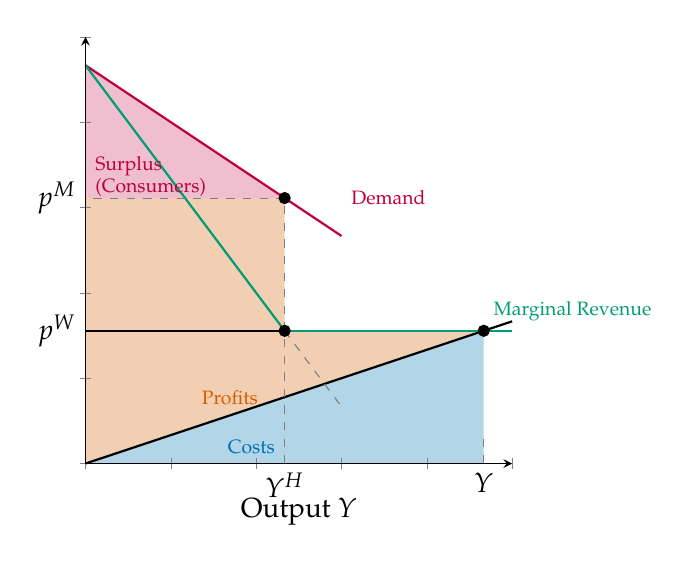
\begin{tikzpicture}
    \pgfmathsetmacro{\A}{7}
    \pgfmathsetmacro{\b}{0.75}
    \pgfmathsetmacro{\m}{1.5}
    \pgfmathsetmacro{\pmax}{\A/\b}          % choke price  (demand intercept)

    \pgfmathsetmacro{\qc}{((\A / \b ) / ( 1/\b + 1/ \m))}
    \pgfmathsetmacro{\pc}{ (\A / \b) - 1/\b * \qc }
    \pgfmathsetmacro{\pw}{\pc}
    \pgfmathsetmacro{\q}{((\A / \b - \pw) / ( 2/\b ))}
    \pgfmathsetmacro{\p}{ (\A / \b) - 1/\b * \q }
    
    
    \begin{axis}[
        xlabel={Output $Y$},
        ymin=0, ymax=10,
        xmin=0, xmax=5,
        yticklabel=\empty,
        xticklabel=\empty,
        axis lines=left,
        enlargelimits=false,
        clip=false,
        axis on top,
        scaled x ticks=false,
        width=7cm, height=7cm,
        title style={font=\bfseries}
    ]

        % profits
        \addplot[fill=red!30, draw=none] coordinates
            {(0,0) (\qc,1/ \m*\qc) (\q,\pw) (\q,\p) (0,\p) (0,0)} -- cycle;
        % costs
        \addplot[fill=blue!30, draw=none] coordinates
            {(0,0) (\qc,\pw) (\qc,0) (0,0)} -- cycle;
        % consumer-surplus
        \addplot[fill=purple!25, draw=none] coordinates
            {(0,\p) (0,\pmax) (\q,\p)} -- cycle;
                    
        \addplot[black, thick, domain=0:5] {\pw};
        \addplot[purple, thick, domain=0:3] {(\A / \b) - 1/\b * x};
        \addplot[black, thick, domain=0:5] {1/\m*x};
        \addplot[green, thick, domain=0:\q] {(\A / \b) - 2/\b * x};
        \addplot[green, thick, domain=\q:5] {\pw};
        \addplot[gray, dashed, domain=\q:3] {(\A / \b) - 2/\b * x};
        %\pgfmathsetmacro{\f}{\p * \q - \q / \m}
        %\addplot[blue, thick, domain=1:5] {1/\m + \f / x};

        
        \addplot[gray, dashed] coordinates {(\q,0) (\q,\p) (0,\p)};
        \addplot[only marks, mark=*, color=black, mark size=2pt] coordinates {(\q,\p)};
        \addplot[only marks, mark=*, color=black, mark size=2pt] coordinates {(\q,\pw)};
        \addplot[gray, dashed] coordinates {(\qc,0) (\qc,1/\m)};
        \addplot[only marks, mark=*, color=black, mark size=2pt] coordinates {(\qc,\pc)};

        %\addplot[gray, dashed] coordinates {(\q,1/\m + \f / \q) (0,1/\m + \f / \q)};
        %\addplot[only marks, mark=*, color=black, mark size=2pt] coordinates {(\q,1/\m + \f / \q)};

        \node[anchor = south west] at (axis cs: 0,{\p+.3}) {\scriptsize \textcolor{purple}{Surplus}};
        \node[anchor = south west] at (axis cs: 0,{\p-.2}) {\scriptsize \textcolor{purple}{(Consumers)}};
        \node[anchor = east] at (axis cs: \q-.2,{1/ \m*\q}) {\scriptsize \textcolor{red}{Profits}};
        \node[anchor = south east] at (axis cs: \q,0) {\scriptsize \textcolor{blue}{Costs}};

        %\node[anchor=south west] at (axis cs: 5,{1/\m+.43}) {\textcolor{blue}{Average Cost}};
        \node[anchor=west] at (axis cs: 3,\p) {\scriptsize \textcolor{purple}{Demand}};
        \node[anchor=south west] at (axis cs: \qc,1/ \m*\qc) {\textcolor{green}{\scriptsize Marginal Revenue}};

        \node[anchor=east] at (axis cs: 0,\p) {$p^{M}$};
        \node[anchor=east] at (axis cs: 0,1/ \m*\qc) {$p^{W}$};

        \node[anchor=north] at (axis cs: \q,0) {$Y^{H}$};
        \node[anchor=north] at (axis cs: \qc,0) {$Y$};

    \end{axis}

    \end{tikzpicture}

 \end{frame}




\begin{frame}{Problems with Perfect Competition}
\Large If price is equal to marginal cost, no firm will undertake the costly research that is
necessary to new products.
\vspace{20pt}

\normalsize

\begin{wideitemize}
    \item Alternative solutions:
    \begin{enumerate}
        \item Public funding of research and innovation (National Science Foundation, National Institute of Health) ‐ reduces impact of fixed cost on AC
        \item Subsidize education in science and engineering ‐ reduces cost of labor to produce ideas, so reduces fixed cost
        \item Prizes for innovators ‐ reduces impact of fixed cost on AC
    \end{enumerate}
\end{wideitemize}
    
\end{frame}



\end{document}
